\chapter{Introduction to Differential Equations}
\begin{fullwidth}
\begin{highlight}
We begin our journey into the world of elementary differential equations by looking at some review.


\section{Review: Precalculus and Calculus}
\begin{weekintro}
  In this section, you will review the techniques from Calculus classes that you should absolutely know in and out: sketching functions, implicit derivatives, and three integration techniques: substitution, by-parts, and partial fractions. \index{integration!by parts} \index{integration!partial fractions} \index{partial fractions} \index{integration by!substitution}
\end{weekintro}

\begin{enumerate}[a)]
    \item Properties of exponents and logarithms
    For $a > 0$, $a \neq 1$, and integers $m, n$ and $x, y > 0$. Then
    \begin{multicols}{3}
    \begin{itemize}
        \item \(a^m \cdot a^n = a^{m+n}\)
        \item \(\frac{a^m}{a^n} = a^{m-n}, \quad (m > n)\)
        \item \((a^m)^n = a^{mn}\)
        \item \((ab)^n = a^n b^n\)
        \item \(\left(\frac{a}{b}\right)^n = \frac{a^n}{b^n}\)
        \item \(a^0 = 1\)
        \item \(a^{-n} = \frac{1}{a^n}\)
        \item \(\ln 1 = 0\)
        \item \(\ln e = 1\)
        \item \(\ln xy = \ln x + \ln y\)
        \item \(\ln \left(\frac{x}{y}\right) = \ln x - \ln y\)
        \item\(\ln x^r) = r \cdot \ln x\)
        \item $\ln(e^x) = x, e^{\ln(x)} = x$
        \item Should be familiar with graphs of the natural exponential and natural logarithm.
    \end{itemize}
    \end{multicols}

    \item Trigonometric Properties
    \begin{multicols}{2}
    \begin{itemize}
        \item \(\sin^2\theta + \cos^2\theta = 1\)
        \item \(1 + \tan^2\theta = \sec^2\theta \)
        \item \(1 + \cot^2\theta = \csc^2\theta\)
        \item \(\sin(\alpha + \beta) = \sin\alpha \cos\beta + \cos\alpha \sin\beta \)
        \item \(\cos(\alpha + \beta) = \cos\alpha \cos\beta - \sin\alpha \sin\beta \)
        \item \(\tan(\alpha + \beta) = \frac{\tan\alpha + \tan\beta}{1 - \tan\alpha \tan\beta}\)
        \item \(\sin(2\theta) = 2\sin\theta \cos\theta \)
        \item \(\cos(2\theta) = \cos^2\theta - \sin^2\theta\)
        \item \(\tan(2\theta) = \frac{2\tan\theta}{1 - \tan^2\theta}\)
    \end{itemize}
    \end{multicols}
    
    \begin{compactitem}
      \item Need to know the values of the trig functions for multiples of $\frac{\pi}{6},\frac{\pi}{4},\frac{\pi}{3},\frac{\pi}{2}$
      \item Need to be familiar with polar coordinates: $x=r\cos(\theta), y=r\sin(\theta)$.
    \end{compactitem}

    \item \textbf{Product rule:} If \(f(x)\) and \(g(x)\) are differentiable functions:
    \[
    \frac{d}{dx}[f(x)g(x)] = f'(x)g(x) + f(x)g'(x)
    \]
    
    \textbf{Example:}  
    \[
    f(x) = x^2 \sin x
    \]
    \[
    f'(x) = (2x)(\sin x) + (x^2)(\cos x) = 2x\sin x + x^2\cos x
    \]

    \item \textbf{Chain rule:} If \(y = f(g(x))\), then:
    \[
    \frac{dy}{dx} = f'(g(x)) \cdot g'(x)
    \]
    
    \textbf{Example:}  
    \[
    y = (3x^2 + 1)^5
    \]
    \[
    \frac{dy}{dx} = 5(3x^2+1)^4 \cdot (6x) = 30x(3x^2+1)^4
    \]

    \item \textbf{Integration by Substitution}
    If $u = g(x)$, then
    \[
    \int f(g(x))g'(x)\,dx = \int f(u)\,du
    \]
    
    \textbf{Example:}  
    \[
    \int 2x \cos(x^2)\,dx
    \]
    Let $u = x^2$, so $du = 2x\,dx$:
    \[
    \int 2x \cos(x^2)\,dx = \int \cos(u)\,du = \sin(u) + C = \sin(x^2) + C
    \]

    \item \textbf{Integration by Parts}
    From the product rule:
    \[
    \int u \, dv = uv - \int v \, du
    \]
    
    \textbf{Example:}  
    \[
    \int x e^x\,dx
    \]
    Let $u = x \implies du = dx$ and $dv = e^x dx \implies v = e^x$:
    \[
    \int x e^x\,dx = x e^x - \int e^x\,dx = x e^x - e^x + C = (x-1)e^x + C
    \]

    \item \textbf{Partial Fraction Decomposition}: 
    If the integrand is a rational function \(\dfrac{P(x)}{Q(x)}\), decompose into simpler fractions.
    
    \textbf{Example:}  
    \[
    \int \frac{1}{x^2 - 1}\,dx
    \]
    Factor denominator:
    \[
    \frac{1}{x^2 - 1} = \frac{1}{(x-1)(x+1)} = \frac{A}{x-1} + \frac{B}{x+1}
    \]
    Multiply through:
    \[
    1 = A(x+1) + B(x-1)
    \]
    Setting $x=1 \implies 1 = 2A \implies A = \tfrac{1}{2}$  
    Setting $x=-1 \implies 1 = -2B \implies B = -\tfrac{1}{2}$
    
    So:
    \[
    \frac{1}{x^2 - 1} = \frac{1}{2}\cdot \frac{1}{x-1} - \frac{1}{2}\cdot \frac{1}{x+1}
    \]
    
    Now integrate:
    \[
    \int \frac{1}{x^2 - 1}\,dx = \frac{1}{2}\ln|x-1| - \frac{1}{2}\ln|x+1| + C
    \]
    \[
    = \frac{1}{2}\ln\left|\frac{x-1}{x+1}\right| + C
    \]
\end{enumerate}
\end{highlight}
\end{fullwidth}

\vspace{2cm}


% \begin{marginfigure}
%   \centering
%   \includegraphics[width=.9\linewidth]{figs/pendulum.JPG}  
%   \caption{Visual representation of pendulum model parameters}
% \end{marginfigure}


\subsection*{In-Class Exercise}

\begin{question}
  Simplify the following expressions:
  \begin{enumerate}[(a)]
  \item \(e^{4 \ln\abs{x+1}} = \)  \solspace{0.3in}
  \item \(\exp\left[ -\frac{1}{2}\ln(x^{2}) \right] = \)  \solspace{0.3in}
  \end{enumerate}
\end{question}
  \solspace{0.3in}


  \begin{question}
    Evaluate the following integrals using substition, integration by parts, and partial fractions, as appropriate.
    \begin{enumerate}[(a)]
    \item \(\int_{0}^{x} x e^{x^{2}}dx\)\footnote{Hint: Substitution} \solspace{0.5in}
    \item \(\int_{1}^{2} x \sin(\pi x)dx\)\footnote{Hint: Integration by parts}  \solspace{0.5in}
    \item \(\int \frac{x}{x^{2}+x-6x}dx\)  \solspace{0.5in}
    \end{enumerate}
  \end{question}

\begin{question}
  Sketch the graph of the function \(f(x) = (x^{2} -4x + 3)e^{-2x}\) \footnote{Determine any minima/maxima, x-intercepts and y-intercepts, and asymptote \(x\to+\infty\) for an accurate sketch.}

      \emptygrid{6}{6}
    \end{question}

\begin{question}
    If \(y(x) = e^{x}\sin(2x)\), evaluate the expression
    \( y''(x) -2 y'(x) + 5 y(x)\).
    Compute the required derivatives\footnote{We use \(y'\) to mean the derivative with respect to the argument, in this case \(dy/dx\). When the function depends on time, say \(x(t)\), then we sometimes additionally use the dot-notation \(\dot{x}=dx/dt\).} first, and then substitute.
    \solspace{1in}
\end{question}


\subsection*{Discussion Problems}
\begin{question}
    Compute the derivative \(y'(x)\) if the following relation between \(y\) and \(x\) holds:
    \[
      \ln\abs{y^{2} + 2} + x^{3}\sin(2x) = C,\: \text{a constant.}
    \]
\end{question}

\begin{question}
    What is the domain of definition of each of the two functions:
    \begin{colenumerate}
      \item \(\ln(2x+1)\)  \item \(\ln\abs{2x+1}\)
    \end{colenumerate}
\end{question}

\begin{question}
    Split the following rational functions into partial fractions:
    \begin{colenumerate}[3]
    \item \(\frac{1}{x^{2} + 4x + 3}\)
    \item \(\frac{2x}{x^{2} + 4x + 3}\)
    \item \(\frac{x^{2}+4x}{x^{2} + 4x + 3}\)
    \end{colenumerate}
    \solspace{0.5in}
\end{question}
  

\begin{question}
    A curve is defined by the implicit expression
    \(
      \cos(2x) + \frac{1}{2}y^{2} = 1.
    \)
    Calculate \textbf{all} the points at which the tangent\footnote{Hint: find the implicit derivative \(y'(x)\)\\ (a) \(y'(x)\to \infty\), (b) \(y'(x)\to \infty\)} to this curve is
    \begin{colenumerate}
      \item Vertical.  \item Horizontal.
    \end{colenumerate}
    \solspace{0.5in}
\end{question}

\begin{question}
    Evaluate the integrals:\footnote{Hint: (a)integration by parts, (b) substitution, (d) substitution/partial fraction, (f) by parts} 
    \begin{colenumerate}[3]
    \item \(\int \ln(x) dx\)
    \item \(\int x e^{x} dx\)
    \item \(\int \frac{x}{x+2} dx\)
    \item \(\int \frac{2x}{x^{2}-4} dx\)
    \item \(\int \frac{x^{2}}{x^{2}+x-6x}dx\)
    \item \(\int e^{x}\sin(\pi x)dx\)
    \end{colenumerate}
    \solspace{0.5in}
\end{question}

%%% Local Variables:
%%% mode: latex
%%% TeX-master: "main"
%%% End:

\section{Basic Terminology \& History}
\subsection{Basic Terminology}
\begin{definition}
       A \emph{differential equation}  is an equation that contains one or more derivatives of an unknown function. 
\end{definition}

A differential equation is an ordinary differential equation (ODE) if it involves an unknown function of only one independent variable.
Example: 
    \[
    \frac{dy}{dt} = -ky.
    \]

A differential equation involving partial derivatives of a function of two or more independent variables is a partial differential equation. 
Example:
    \[
    \frac{\partial u}{\partial t} = \alpha \frac{\partial^2 u}{\partial x^2}.
    \]

Differential equations describe how one quantity changes in relation to other variables.

For a standard algebraic equation, the solution is a number, but for a differential equation, the solution is a function.
\begin{compactitem}
    \item \(y(x)' = y + x^2 +3\) is a differential equation. The unknown function is \( y\)depending on the variable \(x\) and the derivative of \(y\) is involved in the equation.
    \item \(\cos{x} = -1\) is not a differential equation. There is no unknown function.
    \item \(y = x^2 -2x +1\) is not a differential equation since there is no derivative involved.
    \item \(y'(x) = y\) is a differential equation, with unknown function \(y\) with its derivative depending on the variable \(x\).
    \item \(\frac{d}{dx}(\tan{x}) = \sec^2{x}\) is not a differential equation since there is no unknown function
\end{compactitem}

\begin{definition}
    The \emph{order} of a differential equation is the highest derivative that appears in it. 
\end{definition}
\begin{compactitem}
    \item \(\frac{d^2y}{dx^2} + 5 \frac{dy}{dx} + 6y = 0\) is a second-order ODE.
    \item \(y' + 3x^2 =1\) is a first-order ODE.
    \item \(y'' - x^2y' + y = \cos{x}\) is a second-order ODE.
    \item \(y^{4} - xy' + y^2 = 3\) is a fourth-order ODE.
\end{compactitem}


\begin{definition}[Linearity]
    An ODE is \emph{linear} if the dependent variable \(y\) and its derivatives \(y',y'',\ldots,y^n\)  all appear only to the first power and not multiplied together.  
        Example: 
        \[
        a_2(x)y'' + a_1(x)y' + P(x)y = Q(x).
        \]
    An ODE is \emph{nonlinear} if it contains products, powers, or nonlinear functions of the dependent variable or its derivatives.  
        Example:
        \[
        \frac{dy}{dx} = y^2 + \sin(y).
        \]
\end{definition}

\begin{definition}
    A differential equation is homogeneous if all terms depend on the unknown function or its derivatives. If there is a term that does not, it is nonhomogeneous.
    \begin{itemize}
        \item \textbf{Homogeneous}: $\frac{dy}{dx} + p(x)y = 0$
        \item \textbf{Nonhomogeneous}: $\frac{dy}{dx} + p(x)y = q(x)$
    \end{itemize}
\end{definition}

\begin{definition}
    An \emph{Initial Value Problem (IVP)} of an \(n-\)th order differential equation is the differential equation together with an initial condition of \(y\) and the first \(n-1\) derivatives specified at a single point.  
    Example:
    \[
    \frac{dy}{dt} = -ky, \quad y(0)=y_0.
    \]
\end{definition}

\begin{definition}
    A \emph{Boundary Value Problem (BVP):} is a differential equation together with conditions specified at two or more points.  
    Example:
    \[
    \frac{d^2y}{dx^2} + y = 0, \quad y(0)=0, \; y(\pi)=0.
    \]
\end{definition} 

\begin{definition}
    A \emph{solution} of a differential equation is any function that satisfies the differential equation and its initial conditions on some open interval.
\end{definition}
Note that solutions should be accompanied by intervals, since they can provide important information about the solution.\footnote{If \(y\) is a solution to the differential equation, differentiate to obtain \(y'\), then substitute \(y\) and \(y'\) into the differential equation to verify.}
The solution is general if no initial condition is provided.

\begin{example}
    \[
    \frac{dy}{dx} = 2x \quad \Rightarrow \quad y = x^2 + C
    \]  
    is the general solution.  
    If $y(0) = 3$, then $y = x^2 + 3$ is the particular solution.
\end{example}

\begin{question}
Determine whether the given function is a solution of the differential equation.

\begin{enumerate}[a)]
    \item Determine whether $y = e^{2x} + 1$ is a solution of 
    \[
    \frac{dy}{dx} - 2y = -2.
    \]
    
    \item Determine whether $y = \sin(x) + \cos(x)$ is a solution of 
    \[
    \frac{d^2y}{dx^2} + y = 0.
    \]
    
    \item Determine whether $y = x^2$ is a solution of 
    \[
    \frac{dy}{dx} - 2x = 0.
    \]

    \item Determine whether $y = e^{2x}$ is a solution of 
    \[
    \frac{dy}{dx} - 2y = 0.
    \]

    \item  Is \(x=e^{4t}\) a solution to \[x''' - 12x'' + 48x'-64x=0?\]

    \item Is \(y=\sin{t}\) a solution to
    \[
    \left(\frac{dy}{dt}\right)^2 = 1 - y^2?
    \]

    \item Verify that \(x=Ce^{-2t}\) is a solution to \(x' = - 2x\). Find \(C\) to solve for the initial condition \(x(0)=100.\)

    \item Determine whether \(y = x^{-\frac{3}{2}}, y=x^{-\frac{1}{2}}, y=-9x^{-\frac{3}{2}}\), and \(y=7x^{-\frac{1}{2}}-9x^{-\frac{3}{2}}\) are solutions of the differential equation
    \(4x^2y'' + 12xy' + 3y=0,
    \) for \(x>0\).
\end{enumerate}
\end{question}



\subsection{Historical Background}
The study of ODEs is closely tied to the development of calculus and mathematical physics:

\begin{itemize}
    \item \emph{17th Century (Foundations):}  
    The birth of differential equations coincides with the invention of calculus by \emph{Isaac Newton} and \emph{Gottfried Wilhelm Leibniz} in the late 1600s.  
    Newton formulated equations of motion, such as
    \[
    F = ma \quad \Rightarrow \quad m \frac{d^2x}{dt^2} = F(x,t),
    \]
    which is a second-order ODE.

    The Bernoulli brothers also developed methods to solve differential equations to extend the range of their applications

    \item \emph{18th Century (Development):}  
    Mathematicians like \emph{Leonhard Euler}, a student of Johann Bernoulli and \emph{Joseph-Louis Lagrange} developed systematic methods for solving first- and second-order ODEs, as well as studying oscillations, planetary motion, and mechanical systems.  

    \item \emph{19th Century (Theory):}  
    With contributions from \emph{Augustin-Louis Cauchy}, \emph{Sophie Kovalevskaya}, and others, the rigorous theory of existence and uniqueness of solutions was established. The study of linear differential equations and series solutions flourished.

    \item \emph{20th Century (Modern Applications):}  
    Differential equations became essential in physics, engineering, biology, and economics. The qualitative theory of dynamical systems (initiated by \emph{Henri Poincaré}) emphasized studying the behavior of solutions without necessarily finding exact formulas.

    \item \emph{Today:}  
    ODEs remain central in mathematical modeling across disciplines: population dynamics, control systems, epidemiology, neuroscience, climate modeling, finance, etc.
\end{itemize}

Ordinary differential equations provide the mathematical language for describing change.  
From Newton's laws of motion to modern systems biology, ODEs are the foundation of mathematical modeling in the natural and applied sciences.



\section{Mathematical modelling with Differential Equations}
\begin{example}[Newton's Law of Cooling]
Newton's law of cooling states that the rate of change of temperature $T(t)$ of an object is proportional to the difference between the object’s temperature and the ambient temperature $T_a$.  

\[
\frac{dT}{dt} = -k \big(T - T_a\big), \quad k > 0.
\]

\textbf{Solution:}  
This is a first-order linear ODE. We solve it using separation of variables:

\[
\frac{dT}{T - T_a} = -k \, dt.
\]

Integrating both sides:
\[
\ln|T - T_a| = -kt + C.
\]

Exponentiating:
\[
T - T_a = Ce^{-kt}.
\]

Hence the general solution is
\[
T(t) = T_a + (T_0 - T_a)e^{-kt},
\]

where $T_0 = T(0)$ is the initial temperature.
\end{example}

%----------------------------------
% Newton's Cooling Curve
%----------------------------------
\begin{figure}[h]
\centering
\begin{tikzpicture}[scale=0.8]
\begin{axis}[height=0.35\textheight,
    axis lines=middle,
    xlabel={$t$}, ylabel={$T(t)$},
    xmin=0, xmax=8, ymin=72, ymax=102,
    domain=0:8, samples=100,
    thick, smooth, blue
]
\addplot {75 + (100-75)*exp(-0.60*x)}; % Example: Ta=15, T0=60, k=0.5
\draw[dashed, red] (0,75) -- (8,75) node[pos=0.9, below right] {$T_a$};
\end{axis}
\end{tikzpicture}
\caption{Exponential decay of temperature in Newton’s Law of Cooling.}
\end{figure}
%----------------------------------

\begin{example}[Simple Harmonic Oscillator]
The motion of a mass attached to a spring (without damping) is governed by
\[
m \frac{d^2x}{dt^2} + kx = 0,
\]
where $m$ is the mass and $k$ is the spring constant.

\textbf{Solution:}  
Dividing through by $m$ gives
\[
\frac{d^2x}{dt^2} + \omega^2 x = 0, \quad \text{where } \omega = \sqrt{\tfrac{k}{m}}.
\]

This is a second-order linear homogeneous ODE with constant coefficients.  
The characteristic equation is
\[
r^2 + \omega^2 = 0 \quad \Rightarrow \quad r = \pm i\omega.
\]

Hence, the general solution is
\[
x(t) = C_1 \cos(\omega t) + C_2 \sin(\omega t),
\]

which describes oscillatory motion with angular frequency $\omega$.
\end{example}
%----------------------------------
% Simple Harmonic Oscillator
%----------------------------------
\begin{figure}[h!]
\centering
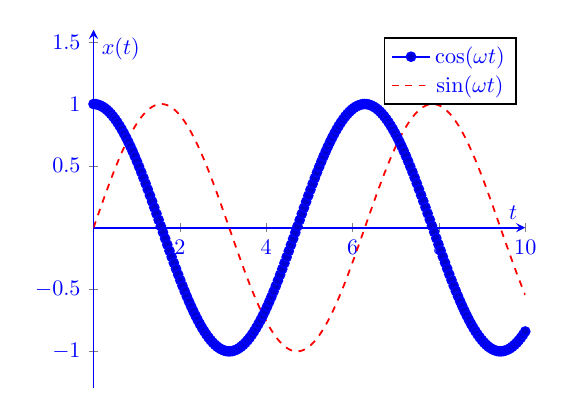
\begin{tikzpicture}[scale=0.8]
\begin{axis}[
    axis lines=middle,
    xlabel={$t$}, ylabel={$x(t)$},
    xmin=0, xmax=10, ymin=-1.3, ymax=1.6,
    domain=0:10, samples=200,
    thick, smooth, blue
]
\addplot {cos(deg(x))}; % x(t) = cos(t)
\addplot[dashed, red] {sin(deg(x))}; % second solution
\legend{$\cos(\omega t)$, $\sin(\omega t)$}
\end{axis}
\end{tikzpicture}
\caption{Solutions of the simple harmonic oscillator.}
\end{figure}
%----------------------------------


\begin{example}[Logistic Population Growth]
A simple model for population growth is given by the logistic equation:
\[
\frac{dP}{dt} = rP \left(1 - \frac{P}{K}\right),
\]

where $r$ is the intrinsic growth rate and $K$ is the carrying capacity.

\textbf{Solution:}  
Separating variables:
\[
\frac{dP}{P(1 - P/K)} = r \, dt.
\]

Using partial fractions:
\[
\frac{1}{P(1 - P/K)} = \frac{1}{P} + \frac{1}{K-P} \cdot \frac{1}{K}.
\]

So,
\[
\int \left( \frac{1}{P} + \frac{1}{K-P} \right) dP = r \int dt.
\]

This gives
\[
\ln|P| - \ln|K-P| = rt + C.
\]

Simplifying:
\[
\ln\left|\frac{P}{K-P}\right| = rt + C.
\]

% Exponentiating:
% \[
% \frac{P}{K-P} = Ce^{rt}.
% \]

\[
\Rightarrow P(t) = \frac{K}{1 + \left(\frac{K}{P_0} - 1\right)e^{-rt}},
\]

where $P_0 = P(0)$.
\end{example}
%----------------------------------
% Logistic Growth Curve
%----------------------------------
\begin{figure}[h]
\centering
\begin{tikzpicture}[scale=0.9]
\begin{axis}[height=0.38\textheight,
    axis lines=middle,
    xlabel={$t$}, ylabel={$P(t)$},
    xmin=0, xmax=12, ymin=0, ymax=90,
    domain=0:12, samples=200,
    thick, smooth, blue
]
\addplot {80/(1 + (80/5 - 1)*exp(-0.6*x))}; % K=80, P0=5, r=0.7
\draw[dashed, red] (0,80) -- (12,80) node[pos=0.9, above] {$K$};
\end{axis}
\end{tikzpicture}
\caption{Logistic growth approaching the carrying capacity $K=80$.}
\end{figure}
%----------------------------------


\section{Slope (Direction) Fields}
\begin{definition}
    A \textbf{slope field} is a graphical representation of a first-order differential equation
    \[
    \frac{dy}{dx} = f(x,y).
    \]
\end{definition}
At each point $(x,y)$ in the plane, a small line segment is drawn with slope $f(x,y)$.

\begin{definition}
    The graph of a solution of a differential equation is called a \emph{solution curve}.
    A curve \(C\) is called an \emph{integral curve} of a differential if every solution curve is a part of it.
\end{definition}
\begin{compactitem}
    \item The slope field provides a qualitative view of solutions without explicitly solving the ODE.
    \item Solution curves are tangent everywhere to the slope field.
\end{compactitem}

\begin{example}[Constant Slope Field]
Consider
\[
\frac{dy}{dx} = 1.
\]
Every line segment has slope $1$ (a $45^\circ$ line).  
Solution curves are lines of the form

$y = x + C$.
\begin{center}
\begin{tikzpicture}
\begin{axis}[
    width=7cm, height=7cm,
    axis x line=middle, axis y line=middle,
    xlabel={$x$}, ylabel={$y$},
    xmin=-2, xmax=2, ymin=-2, ymax=2,
    samples=15, domain=-2:2, domain y=-2:2
]
% slope field with constant slope dy/dx = 1
\addplot[blue, quiver={u=1, v=1, scale arrows=0.15}, -stealth] {0};
\end{axis}
\end{tikzpicture}
\end{center}
\end{example}

\begin{example}[Non-constant Slope Field]
We visualize the slope field for
\[
\frac{dy}{dx} = x.
\]

\begin{center}
\begin{tikzpicture}
\begin{axis}[
    width=8cm, height=8cm,
    axis x line=middle, axis y line=middle,
    xlabel={$x$}, ylabel={$y$},
    xmin=-2, xmax=2, ymin=-2, ymax=2,
    samples=15, domain=-2:2, domain y=-2:2
]
% slope field
\addplot[blue, quiver={u=1,v={x},scale arrows=0.2},-stealth] {0};
\end{axis}
\end{tikzpicture}
\end{center}


The general solution is:
\[
y = \frac{x^2}{2} + C
\]
which agrees with the slope field.
\end{example}

\begin{example}[Logistic Growth]
Consider the logistic ODE:
\[
\frac{dy}{dx} = y(1-y).
\]
\begin{itemize}
    \item When $0 < y < 1$, slopes are positive (growth).  
    \item When $y > 1$, slopes are negative (decay).  
    \item $y=0$ and $y=1$ are equilibrium solutions.
\end{itemize}

\end{example}


\begin{figure}[htb]
    \centering
    \begin{minipage}[t]{0.48\textwidth}
        \centering
        \begin{tikzpicture}
            \begin{axis}[
                width=7cm, height=7cm,
                axis x line=middle, axis y line=middle,
                xlabel={$x$}, ylabel={$y$},
                xmin=-2, xmax=2, ymin=-1, ymax=2,
                samples=15, domain=-2:2, domain y=-1:2
            ]
            % slope field for dy/dx = y(1-y)
            \addplot[blue, quiver={u=1, v={y*(1-y)}, scale arrows=0.15}, -stealth] {0};
            \end{axis}
        \end{tikzpicture}
        % \captionof{figure}{Slope field for $y' = y(1-y)$ using `pgfplots`.}
    \end{minipage}%
    \hfill
    \begin{minipage}[t]{0.48\textwidth}
        \centering
        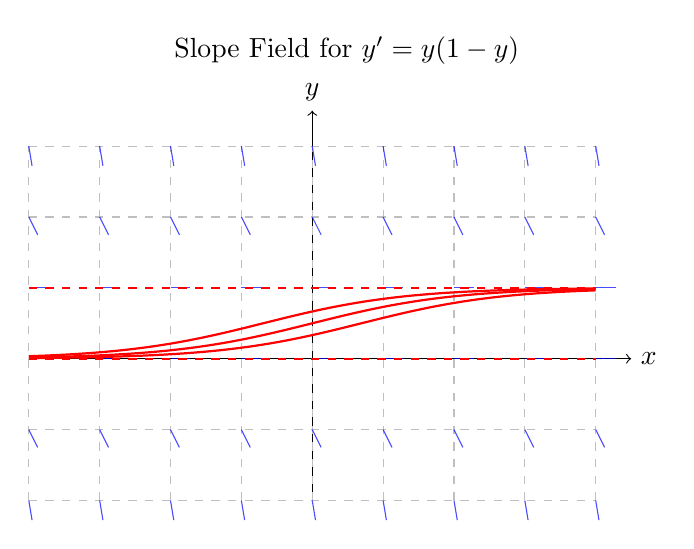
\begin{tikzpicture}[scale=0.9]
            % Define the plotting area
            \def\xmin{-4}
            \def\xmax{4}
            \def\ymin{-2}
            \def\ymax{3}
            \draw[->] (\xmin, 0) -- (\xmax + 0.5, 0) node[right] {$x$};
            \draw[->] (0, \ymin) -- (0, \ymax + 0.5) node[above] {$y$};

            % Draw grid lines
            \draw[dashed, gray!50] (\xmin, \ymin) grid (\xmax, \ymax);

            % Loop to draw the slope field for y' = y(1-y)
            \foreach \x in {\xmin,...,\xmax} {
                \foreach \y in {\ymin,...,\ymax} {
                    \pgfmathsetmacro{\slope}{\y*(1-\y)} % slope field formula
                    \pgfmathsetmacro{\angle}{atan(\slope)} % direction angle
                    \draw[blue, opacity=0.7] (\x, \y) -- ++(\angle:8pt);
                }
            }

            % Plot example integral curves (solutions to logistic equation)
            % General solution: y(x) = 1/(1 + Ce^{-x})
            \draw[red, thick, domain=\xmin:\xmax, samples=200, smooth]
                plot (\x,{1/(1+exp(-\x))});
            \draw[red, thick, domain=\xmin:\xmax, samples=200, smooth]
                plot (\x,{1/(1+2*exp(-\x))});
            \draw[red, thick, domain=\xmin:\xmax, samples=200, smooth]
                plot (\x,{1/(1+0.5*exp(-\x))});

            % Equilibria lines y=0 and y=1
            \draw[dashed, thick, red] (\xmin,0)--(\xmax,0);
            \draw[dashed, thick, red] (\xmin,1)--(\xmax,1);

            % Add title (can be moved to a single overall caption)
            \node[above] at (current bounding box.north) {Slope Field for $y' = y(1-y)$};
        \end{tikzpicture}
        % \captionof{figure}{Slope field and solution curves using `tikzpicture` loops.}
    \end{minipage}
    \caption{Slope field and some solution curves for the logistic equation. Equilibria occur at $y=0$ and $y=1$.
    Play around with the sage code here \url{https://shorturl.at/K9f7l}}
\end{figure}


\begin{example}
For the differential equation,
\[
\frac{dy}{dx} =\frac{x}{y},
\]
\end{example}
\begin{figure}[h]
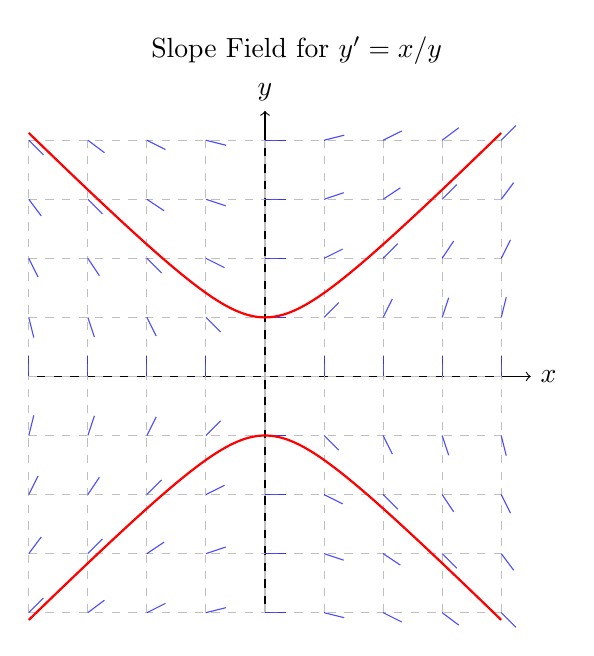
\begin{tikzpicture}[scale=0.75]
    % Define the plotting area
    \def\xmin{-4}
    \def\xmax{4}
    \def\ymin{-4}
    \def\ymax{4}
    \draw[->] (\xmin, 0) -- (\xmax + 0.5, 0) node[right] {$x$};
    \draw[->] (0, \ymin) -- (0, \ymax + 0.5) node[above] {$y$};

    % Draw grid lines
    \draw[dashed, gray!50] (\xmin, \ymin) grid (\xmax, \ymax);

    % Loop to draw the slope field
    \foreach \x in {\xmin, ..., \xmax} {
        \foreach \y in {\ymin, ..., \ymax} {
            % Conditional to handle the division by zero
            \pgfmathsetmacro{\yval}{\y}
            \ifdim\y pt = 0pt
                % Slope is undefined, so draw a vertical segment (if x is not 0)
                \ifdim\x pt = 0pt
                    \relax % Do nothing at the origin
                \else
                    \draw[blue, opacity=0.7] (\x, \y) -- ++(90:10pt); % vertical
                \fi
            \else
                % Normal calculation for all other points
                \pgfmathsetmacro{\angle}{atan(\x/\y)}
                \draw[blue, opacity=0.7] (\x, \y) -- ++(\angle:10pt);
            \fi
        }
    }
    
    % Draw one of the integral curves (a hyperbola for y^2 - x^2 = 1)
    \draw[red, thick, domain=-4:4, samples=101, smooth, no markers] plot (\x, {sqrt(1+\x*\x)});
    \draw[red, thick, domain=-4:4, samples=101, smooth, no markers] plot (\x, {-sqrt(1+\x*\x)});

    % Add title
    \node[above] at (current bounding box.north) {Slope Field for $y' = x/y$};
\end{tikzpicture}
\caption{
    An \emph{integral curve} is more general term for the graph of a solution, including those that are not functions. For example, the full hyperbola \(y^{2}-x^{2}=K\) is an integral curve, but the upper branch (\(y=\sqrt{x^{2}+K}\)) and lower branch (\(y=-\sqrt{x^{2}+K}\)) are the individual solution curves.}
\end{figure}


\begin{compactitem}
    \item Slope fields help visualize the qualitative behavior of solutions.
    \item Equilibrium solutions correspond to horizontal slopes ($f(x,y)=0$).
    \item They are especially useful when an ODE cannot be solved analytically.
\end{compactitem}


\subsection{Practice Problems}
\begin{question}
  Give definitions of the following terms and/or answer the questions\footnote{research it if we did not discuss it in class.}:
  \begin{enumerate}[(a)]
    \item \textbf{Define} an equilibrium of a \ode{}.\index{equilibrium} \solspace{.25in}
    \item \textbf{Explain} the procedure for calculating equilibria. \solspace{.25in}
    \item \textbf{Explain} the difference between a \emph{general} and  \emph{particular} solution.\index{solution!general} \index{solution!particular} \solspace{.25in}
  \end{enumerate}
\end{question}

\begin{question}Show that out of three functions Provided
  two are solutions of the \ode{} 
  
  \mbox{\( x^{2}\, y''(x) - x\,y'(x) + y(x) = 0\)}, and the third is not.\index{solution!verifying}
  \begin{colenumerate}[3]
   \item \(y_{1}(x) = \ln(x)\)
   \item \(y_{2}(x) = x\ln(x)\)
   \item \(y_{3}(x) = x-x\ln(x)\)
  \end{colenumerate}
\end{question}
% \vfill



\begin{subsection}{Summary}
    \begin{enumerate}
        \item A differential equation relates a function to its derivatives.
        \item The order of a differential equation is the highest derivative present.
        \item A solution of a differential equation is a function that satisfies the equation.
        \item Initial value problems specify conditions at a single point, while boundary value problems specify conditions at multiple points.
        \item Mathematical modeling uses differential equations to describe real-world phenomena.
        \item Historical development of differential equations is closely tied to calculus and physics.
        \item Slope fields visualize solutions qualitatively.
    \end{enumerate}